\documentclass{article}
\usepackage{graphicx} % Required for inserting images
\usepackage[top=0.9in, bottom=1in, left=1.5in, right=1.5in]{geometry}
\usepackage[utf8]{inputenc}
\usepackage[icelandic]{babel}
\usepackage[T1]{fontenc}
\usepackage[sc]{mathpazo}
\usepackage[parfill]{parskip}
\renewcommand{\baselinestretch}{1.2}
% Tables and lists
\usepackage{booktabs,tabularx}
\usepackage{multirow}
\usepackage{enumerate}
\usepackage{adjustbox}
\usepackage{multicol}
\usepackage{xcolor}
\usepackage{algpseudocode}
\usepackage{tikz}
\usepackage{nicefrac}
\usepackage{changepage}
\usetikzlibrary{arrows, positioning, calc, graphs}

% Math
\usepackage{amsmath, amsfonts, amssymb, amsthm}
% Graphics

\usepackage{graphicx}
\usepackage{tikz}
% Code environment
\usepackage{minted}
%\usepackage{bm}
%\usepackage{siunitx}
%\usepackage{animate}
%\usepackage{hyperref}
%\usepackage{movie15}
%\usepackage{multicol}
%\usepackage{changepage}
\title{Forritunarmál Hópverkefni 4}
\author{Ragnar Björn Ingvarsson, rbi3 \\
		Daníel Snær Halldórsson, dsh11 \\
		Ólafur Sær Sigursteinsson, oss27 \\
		Jonathan Jakub Otuoma, jjo1}
\tikzset{->, >=stealth', shorten >=1pt, node distance=2cm,thick, main node/.style={circle,draw,minimum size=3em}}

\begin{document}
\renewcommand\thepage{}
	
	\maketitle

	\newpage
	\setcounter{page}{1}
	\renewcommand\thepage{\arabic{page}}

	\section{}
	\begin{verbatim}
;; Notkun: (myiota n)
;; Fyrir: n er heiltala, n>=0
;; Gildi: Listi allra heiltalna i, þannig að
;; 0 < i <= n, í vaxandi röð,
;; þ.e. listinn (1 2 ... n)
(define (myiota n)
;; Notkun: (hjalp r x)
;; Fyrir: r er heiltala, 0 <= r <= n.
;; x er listinn (r+1 r+2 ... n)
;; Gildi: Listinn (1 2 ... n)
(define (hjalp r x)
  (if (= r 0)
      x
      (hjalp (- r 1) (cons r x))
      )
)
(hjalp n '())
)
	\end{verbatim}
	\begin{center}
		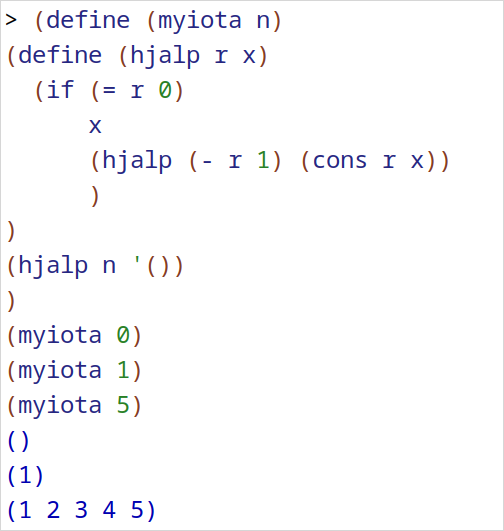
\includegraphics[scale=0.35]{myiota.png}
	\end{center}

	\newpage
	\section{}
	\begin{verbatim}
;; Notkun: (myfoldl f u x)
;; Fyrir: f er tvíundarfall, þ.e. fall
;; sem tekur tvö viðföng af einhverju
;; tagi, x er listi (x1 ... xN)
;; gilda af því tagi, u er gildi
;; af því tagi.
;; Gildi: (f (f ...(f (f u x1) x2) ...) xN)
;; Aths.: Með öðrum orðum, ef við skilgreinum
;; tvíundaraðgerð ! með a!b = (f a b),
;; þá er útkoman úr fallinu gildið á
;; u ! x1 ! x2 | ... ! xN
;; þar sem reiknað er frá vinstri til
;; hægri
(define (myfoldl f u x)
  (if (null? x)
      u
      (myfoldl f (f u (car x)) (cdr x))
  )
)
	\end{verbatim}
	\begin{center}
		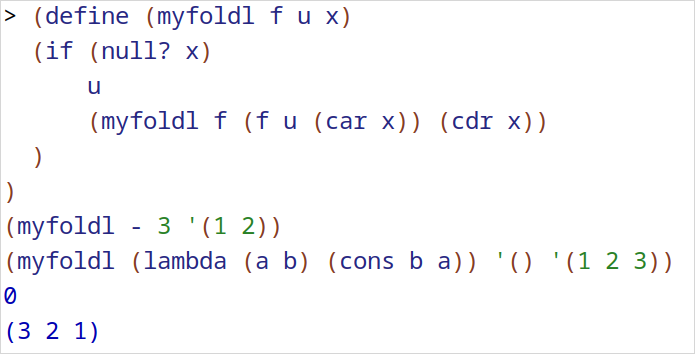
\includegraphics[scale=0.35]{myfoldl.png}
	\end{center}

	\section{}
	\begin{verbatim}
(myfoldl + 0 (myiota 30))
(myfoldl * 1 (myiota 30))
	\end{verbatim}
	\begin{center}
		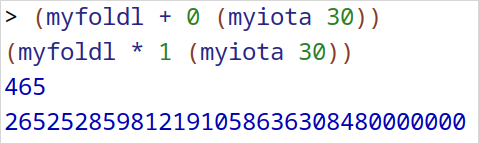
\includegraphics[scale=0.35]{30.png}
	\end{center}
\end{document}
